\documentclass{standalone}
\usepackage{tikz}
\begin{document}
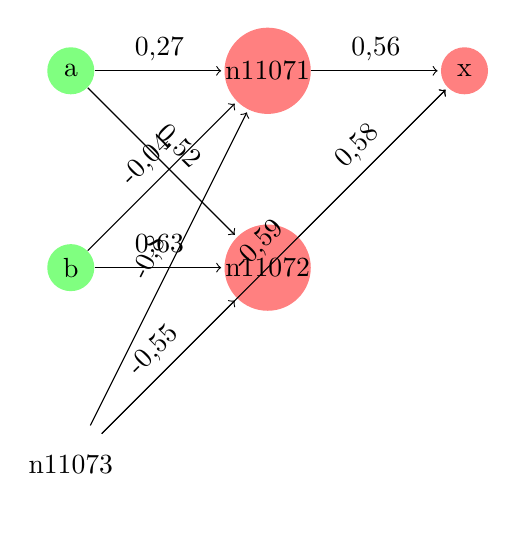
\begin{tikzpicture}[shorten >=1pt,->,draw=black!,node distance=2.5cm]
\tikzstyle{neuron}=[circle,fill=black!25,minimum size=17pt,inner sep=0pt]
\tikzstyle{constant}=[neuron, fill=white!50];
\tikzstyle{identity}=[neuron, fill=green!50];
\tikzstyle{sigmoid}=[neuron, fill=red!50];
\node [identity] (a) {a};
\node [identity,below of=a] (b) {b};
\node [constant,below of=b] (n11073) {n11073};
\node [sigmoid,right of=a] (n11071) {n11071};
\node [sigmoid,below of=n11071] (n11072) {n11072};
\node [sigmoid,right of=n11071] (x) {x};
\path[every node/.style={sloped,anchor=south,auto=false}]
(a) edge node {0,27} (n11071)
(a) edge node {0,52} (n11072)
(n11073) edge node {-0,8} (n11071)
(n11073) edge node {-0,55} (n11072)
(n11073) edge node {-0,59} (x)
(n11071) edge node {0,56} (x)
(b) edge node {0,63} (n11072)
(b) edge node {-0,04} (n11071)
(n11072) edge node {0,58} (x)
;\end{tikzpicture}
\end{document}